\chapter{Modellansichten}
\label{app:modelle}

\begin{sidewaysfigure}
  \centering
  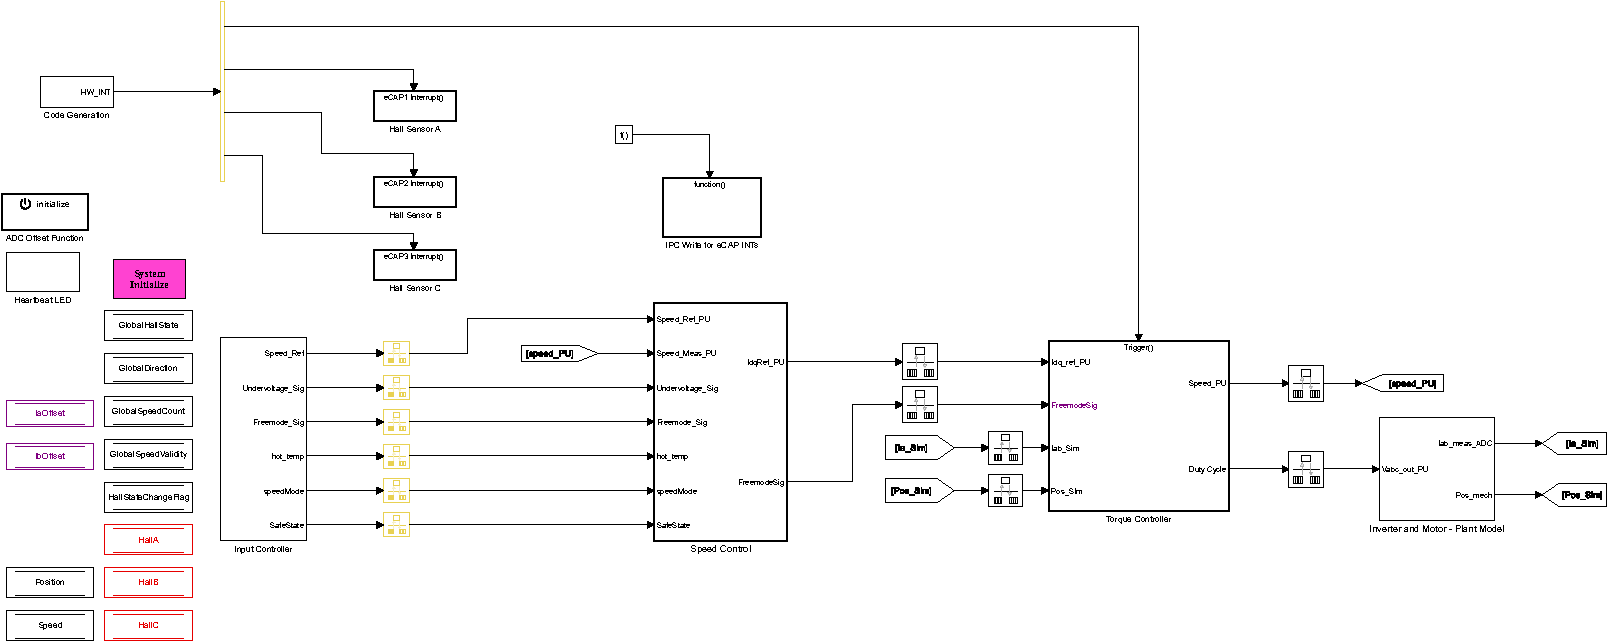
\includegraphics[width=\linewidth]{impmodel_top}
  \caption{Oberste Ebene des Modells \datei{impmodel.slx} aus \cite{akguel2023},
    unveränderte Ansicht aus Simulink}
  \label{fig:impmodel_orig}
\end{sidewaysfigure}

\chapter{Übersicht der Werkzeugskripte}
\label{app:skripte}
% Tabelle matlab/tools/*.m: Skript, Zweck, Schritt/Commit
\offen{Tabelle}

\chapter{Änderungsverlauf}
\label{app:verlauf}
% Tags P1a, P1b, P1b.1 und wichtige Commits mit Kurzbeschreibung
\offen{Tabelle}

\chapter{Konfigurationsparameter}
\label{app:parameter}
% Auszug foc_config: ctrl_limits, PU-Basis, Messkette, Profile im Vergleich
\offen{Tabelle}
